% \documentclass{article}
% \usepackage[utf8]{inputenc}
% \usepackage{fullpage}
% \usepackage {setspace}
% \usepackage[hang,flushmargin]{footmisc} %control footnote indent
% \usepackage{url} % for website links
% \usepackage{amssymb,amsmath}%for matrix
% \usepackage{graphicx}%for figure
% \usepackage{appendix}%for appendix
% \usepackage{float}
% \floatstyle{plaintop}
% \restylefloat{table}
% \usepackage{multirow}
% \usepackage{longtable}
% \usepackage{morefloats}%in case there are too many float tables and figures
% \usepackage{caption}
% \usepackage{subcaption}
% \usepackage{listings}
% \captionsetup[subtable]{font=normal}
% \usepackage{color}
% \usepackage{hyperref}
% \usepackage[round]{natbib}
% \usepackage{algorithm}
% \usepackage{algorithmicx}
% \usepackage[noend]{algpseudocode}

% \makeatletter
% \def\BState{\State\hskip-\ALG@thistlm}
% \makeatother

% %\usepackage{Sweave}
% \setlength{\parindent}{0em}
% \setlength{\parskip}{0.5em}


% \graphicspath{{0.plots/}}



% \begin{document}

\section{Statistical Methods}
Three major statistical methods that will be used, including Bayesian quantile regression, JM uses longitudinal quantile regression and dynamic prediction method for the probabilities of future events based on JM of longitudinal and survival data.

\subsection{Bayesian Quantile Regression}
\subsubsection{Quantile Regression and Asymmetric Laplace Distribution}\label{sec:QRALD}%%%%%

Let $Y$ be a real valued random variable with cumulative distribution function $F_Y(y) = P(Y \le y)$. By definition, the $\tau$th quantile of $Y$, where $\tau\in[0,1]$,  is given by
\begin{equation}\label{eqn:quantile}
Q_{Y}(\tau)=F_{Y}^{-1}(\tau)=\inf\left\{ y:F_{Y}(y)\geq\tau\right\}
\end{equation}

In contrast to mean regression (or linear regression), quantile regression models the conditional quantile of the outcome $Y$ given a set of covariates, which is defined as

\begin{equation}\label{eqn:lqr}
Q_{Y|{\boldsymbol X}}(\tau)={\boldsymbol X}^{\top}\boldsymbol{\beta}_{\tau}
\end{equation}

Given the data sample, the estimates of the regression coefficients at $\tau$th quantile can be obtained by solving 

\begin{equation}\label{eqn:loss_fun}
\hat{\boldsymbol{\beta}}_{\tau}=\underset{\boldsymbol{\beta}\in \mathbb{R}^{p}}{\mbox{arg min}}\sum_{i=1}^{n}\left[\rho_{\tau}(Y_{i}-{\boldsymbol X}_i^{\top}\boldsymbol{\beta})\right],
\end{equation}

where the loss function $\rho_{\tau}(\cdot)$ is defined as $\rho_{\tau}(Y)=Y(\tau-{I}{(Y<0)}).$ \par

However, there is no direct solution to (\ref{eqn:loss_fun}), rather the minimization problem can be reformulated as a linear programming problem, where simplex methods or interior point methods can be applied to solve for the estimates \citep{koenker2005quantile}. The minimization problem can also be rephrased as a maximum-likelihood problem by using the asymmetrical Laplace distribution (ALD). \citep{koenker1999goodness,yu2001bayesian}.\par


Suppose a random variable $Y$ follows ALD($\mu, \sigma, \tau$), then the probability density function of $Y$ can be written as

\begin{equation}\label{eqn:ald}
f(Y|\mu, \sigma, \tau)=\frac{\tau(1-\tau)}{\sigma}\exp\left[-\rho_{\tau}\left(\frac{Y-\mu}{\sigma}\right)\right],
\end{equation}

where $\mu\in(-\infty, \infty)$ is the location parameter, $\sigma$ is the scale parameter and $\tau\in(0, 1)$ is the skewness parameter. Thus, in a standard linear model

\begin{equation}\label{eqn:lm}
Y_i={\boldsymbol X_i}^{T}\boldsymbol{\beta}+\varepsilon_i,
\end{equation}

if we assume the random error $\varepsilon_i\sim$ ALD($0, \sigma, \tau$), then $Y_i|{\boldsymbol X}_i\sim$
ALD(${\boldsymbol X_i}^{\top}\boldsymbol{\beta}, \sigma, \tau$), that is the likelihood function can be written as

\begin{equation}\label{eqn:yald}
L(\boldsymbol{\beta}, \sigma; {\boldsymbol Y}, \tau)\propto\frac{1}{\sigma^n}\exp\left[-\sum_{i=1}^n\rho_{\tau}\left(\frac{Y_i-{\boldsymbol X_i}^{\top}\boldsymbol{\beta}}{\sigma}\right)\right].
\end{equation}

If we treat $\sigma$ in (\ref{eqn:yald}) as nuisance then the maximization of (\ref{eqn:yald}) with respect to $\boldsymbol{\beta}$ is exactly the same as that in (\ref{eqn:loss_fun}).

\begin{figure}[H]
\label{fig:ald_ld}
\begin{center}
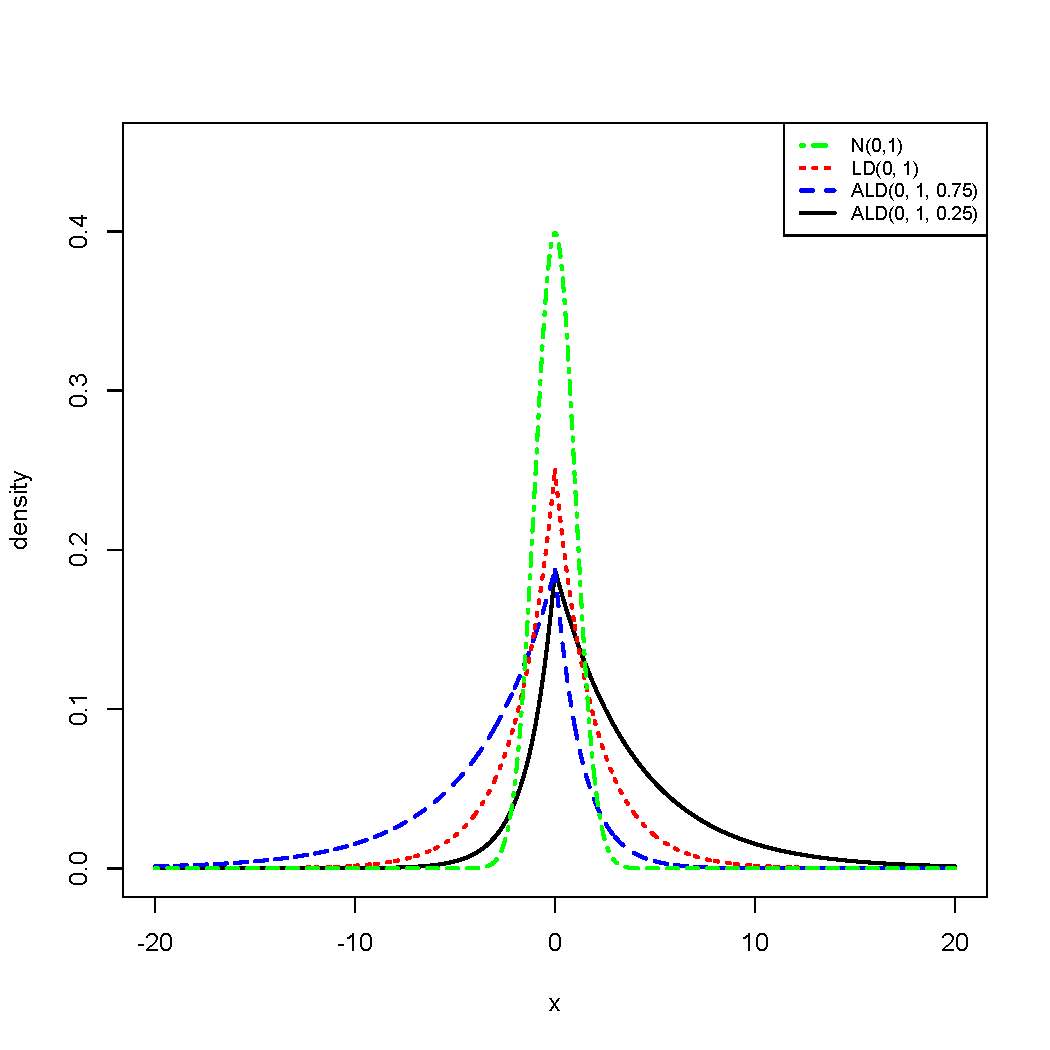
\includegraphics[scale=0.45]{ald_ld_normal.pdf}
\caption{Graphical visualization of ALD versus Laplace distribution (LD) and standard normal distribution.}
\end{center}
\end{figure}


\subsubsection{Bayesian Linear Quantile Mixed Model}\label{sec:BLQMM}%%%%%

As a natural extension to linear quantile regression, when working on longitudinal data, linear quantile mixed model (LQMM) is defined as
\begin{equation}\label{eqn:lqmm}
Q_{Y_{ij}|{\boldsymbol X}_{ij},{\boldsymbol Z}_{ij}}(\tau)={\boldsymbol X}_{ij}^{\top} \boldsymbol{\beta}+ {\boldsymbol Z}_{ij}^{\top}\boldsymbol{u}_i,\ i=1, \cdots, N;\ j=1,\cdots, n_i.
\end{equation}
where $Y_{ij}$ is the response variable for subject $i$ at time $j$, ${\boldsymbol X}_{ij}$ is the $p-$dimensional fixed effects covariates and $\boldsymbol{\beta}_{\tau}$ is the corresponding $p\times1$ vector of fixed effects, while ${\boldsymbol Z}_{ij}$ is the $k-$dimensional random effects covariates and $\boldsymbol{u}_i$ is the corresponding $k\times 1$ vector of random effects for subject $i$. Under the assumption that the random error follows ALD$(0, \sigma, \tau)$, conditional on the random effects $\boldsymbol{u}_i$, $Y_{ij}$'s are independently and identically distributed as ALD(${\boldsymbol X}_{ij}^{\top}\boldsymbol{\beta}+{\boldsymbol Z}_{ij}^{\top}\boldsymbol{u}_i, \sigma, \tau$):

\begin{equation}\label{eqn:ald_lqmm}
f(Y_{ij}|\boldsymbol{\beta},\boldsymbol{u}_i,\sigma)=\frac{\tau(1-\tau)}{\sigma}\exp\left[-\rho_{\tau}\left(\frac{Y_{ij}-{\boldsymbol X}_{ij}^{\top}\boldsymbol{\beta}-{\boldsymbol Z}_{ij}^{\top}\boldsymbol{u}_i}{\sigma}\right)\right]
\end{equation}

To develop a Gibbs sampler for model (\ref{eqn:ald_lqmm}), we need to assume a location-scale mixture representation of the ALD \citep{kotz2001laplace}. Under such assumption the random error is represented as $\varepsilon_{ij}=\kappa_1e_{ij}+\kappa_2\sqrt{\sigma e_{ij}}v_{ij}$,

where \[\kappa_1=\frac{1-2\tau}{\tau(1-\tau)}, \mbox{ and } \kappa_2^2=\frac{2}{\tau(1-\tau)},\]
and \[v_{ij}\sim N(0,1), \mbox{ and } e_{ij}\sim\exp(\sigma).\]

As a result, the linear mixed model is then reparameterized as
\begin{equation}\label{eqn:reformald2}
Y_{ij}={\boldsymbol X}_{ij}^{\top}\boldsymbol{\beta}+{\boldsymbol Z}_{ij}^{\top}\boldsymbol{u}_i+\kappa_1e_{ij}+\kappa_2\sqrt{\sigma e_{ij}}v_{ij},
\end{equation}


or equivalently
\begin{equation}\label{eqn:lo_sc_lh}
f(Y_{ij}|\boldsymbol{\beta},\boldsymbol{u}_i,e_{ij},\sigma)=\frac{1}{\sqrt{2\pi\kappa_2^2\sigma e_{ij}}}\exp\left[-\frac{1}{2\kappa_2^2\sigma e_{ij}}(Y_{ij}-{\boldsymbol X}_{ij}^{\top}\boldsymbol{\beta}-{\boldsymbol Z}_{ij}^{\top}\boldsymbol{u}_i-\kappa_1e_{ij})^2\right].
\end{equation}


Following (\ref{eqn:reformald2}), a fully specified Bayesian model would include follows:

\begin{eqnarray*}
&& {\boldsymbol v}\sim\prod_{i=1}^N\prod_{j=1}^{n_i}\exp\left(-\frac{v_{ij}^2}{2}\right),\\
&& {\boldsymbol e}\sim\prod_{i=1}^N\prod_{j=1}^{n_i}\frac{1}{\sigma}\exp\left(-\frac{e_{ij}}{\sigma}\right),\\
&& \boldsymbol{\beta} \sim MVN_p({\boldsymbol 0}, \boldsymbol{\Sigma}),\\
&& \boldsymbol{u}_i|\eta \sim MVN_p({\boldsymbol 0}, \eta^2\boldsymbol{I}),\\
&& \sigma\sim IG(a_0, b_0),\\
&& \eta\sim IG(c_0, d_0).
\end{eqnarray*}



\subsection{Longitudinal Quantile Regression and Joint Modeling}
Following \cite{Alessio2014qrjm}, we extend the traditional joint modeling (JM) of longitudinal and survival data by using the longitudinal quantile mixed model in place of the linear mixed model.\par

In the time-to-event data let $T_i=min(T_i^*, C_i)$ be the observed event time for subject $i\ (i=1, \cdots, n)$, where $T_i^*$ is the true underlying event time and $C_i$ is the censoring time. Let $\Delta_i$ be the event indicator and define it as $\Delta_i = I(T_i^* < C_i)$, where $I(\cdot)$ is the indicator function. If $\Delta_i=1$, i.e. $T_i^* < C_i$, we say an event is observed during the study period; in contrast, when $\Delta_i=0$ there is no event observed until the end of the study or when the patient is lost follow-up (i.e. censored).\par

While in the longitudinal part, let $Y_{it}$ be the continuous longitudinal outcome for subject $i\ (i=1, \cdots, n)$ measured at time $t\ (t=1, \cdots, n_i)$. Note that we can only observe $Y_{it}$ when $t\le T_i$, so the longitudinal outcome for subject $i$ can be written as ${\boldsymbol Y}_i=\{Y_{it}: t\le T_i\}$.\par

There is also a set of covariates in the model. In the longitudinal model, let $\boldsymbol{X}_{it}$ and $\boldsymbol{H}_{it}$ be the fixed effects covariates that are associated with the outcome and $\boldsymbol{Z}_{it}$ be the covariates associated with $k-$dimensional random effects $\boldsymbol{u}_i$; in the time-to-event model, we have $\boldsymbol{W}_{i}$ as the fixed effects covariates that are only associated with event time (not longitudinal outcome) and this model shares the same fixed effects covariates $\boldsymbol{H}_{it}$ and random effects covariates $\boldsymbol{Z}_{it}$ with the longitudinal model. Thus the two models are related by sharing some of the fixed and random variables, and the degree of associations from those two sources of measurements (observed and unobserved) are measured by another two parameters $\alpha_1$ and $\alpha_2$, respectively.\par


The proposed JM as described above can be written as a set of two models:

\begin{equation}\label{eqn:joint}
\left\{
\begin{array}{l}
Y_{it} = {\boldsymbol X}_{it}^{\top}\boldsymbol{\beta} + {\boldsymbol H}_{it}^{\top}\boldsymbol{\delta} + {\boldsymbol Z}_{it}^{\top}{\boldsymbol u}_i + \varepsilon_{it}, \varepsilon_{it}\sim ALD(0, \sigma,\tau)\\
h(T_i|\mathcal{T}_{iT_i}, {\boldsymbol W}_i;  \boldsymbol{\gamma}, \alpha_1, 
\alpha_2) = h_0(T_i)\exp({\boldsymbol W}_i^{\top}\boldsymbol{\gamma} + \alpha_1{\boldsymbol H}_{iT_i}^{\top}\boldsymbol{\delta} + \alpha_2{\boldsymbol Z}_{iT_i}^{\top}{\boldsymbol u}_{i})
\end{array}
\right.
\end{equation}

where the first equation is the linear quantile mixed model discussed in Section \ref{sec:BLQMM} and the second equation takes the format of Cox proportional hazards model where $h_0(\cdot)$ is the baseline hazard function.\par

Individual heterogeneity is captured by the term ${\boldsymbol Z}_{it}^{\top}{\boldsymbol u}_i$ in the model, which is the deviation of subject $i$ from the population average. Note that the posterior estimates of the random effects can be used to draw subject specific predictions of future event probabilities or longitudinal outcome when the subject is from the study population that we used to fit the model.\par

Also note that in quantile regression, the parameter estimates are functions of the quantile. This is also true in the proposed JM. That is, parameters in the survival models like $\boldsymbol{\gamma}$ also vary according to different values of $\tau$. Depending on research aims, different strategies may be taken to utilize the flexibility of the model. For example, if we are interested in the complete distribution of parameter estimates as a function of quantile, we can just run the model through the range of possible quantiles, collect and compare the results from different quantiles of the outcome. Less varying values of the estimate indicates a relatively stable effect from the corresponding covariate on the outcomes.  In contrast, if the interest only lies in investigating the effect of lower or higher quantile for the longitudinal outcome on the survival probabilities as discussed in Section \ref{sec:bak_lqm_jm}, we may just fix the quantile to a specific value and conduct the analysis. 

% need to add more model explanation and interpretation here, for example 
% how it can be used to make future predication, 
% all the parameter estimations depend on quantile.
% interpretation of random effects factors


\subsubsection{The Survival Model}
As the details for the longitudinal model has been discussed previously in Section \ref{sec:BLQMM}, here we only focus on the survival component of the JM. \par

For subject $i$, the complete survival likelihood can be written as:

\begin{eqnarray}\label{eqn:survival_like}\label{eqn:lik_sur}
f(T_i, \Delta_i|\boldsymbol{u_i})&=&f(T_i|\mathcal{T}_{iT_i}, \boldsymbol{W}_i)^{\Delta_i}S(T_i|\mathcal{T}_{iT_i}, \boldsymbol{W}_i)^{1-\Delta_i}\\
&=&\nonumber h(T_i|\mathcal{T}_{iT_i}, \boldsymbol{W}_i)^{\Delta_i}S(T_i|\mathcal{T}_{iT_i}, \boldsymbol{W}_i)^{1-\Delta_i},
\end{eqnarray}
where $h(T_i|\mathcal{T}_{iT_i}, \boldsymbol{W}_i)$ is given in (\ref{eqn:joint}) and $S(\cdot)$ is the survival function, i.e.

\begin{equation}\label{eqn:survival}
S(T_i|\mathcal{T}_{iT_i}, \boldsymbol{W}_i)=\exp\left\{-\int_0^{T_i}h_0(s)\exp({\boldsymbol W}_i^{\top}\boldsymbol{\gamma} + \alpha_1{\boldsymbol H}_{is} ^{\top}\boldsymbol{\delta}+ \alpha_2{\boldsymbol Z}_{is}^{\top}{\boldsymbol u}_i)ds\right\}.
\end{equation}

For the baseline hazard $h_0(s)$, parametric form like Weibull model can be used or it can be left unspecified. However, the choice of baseline hazard is not a main focus of the this project.



\subsubsection{Complete Likelihood Function and Bayesian Inference}\label{sec:estimation}


The complete joint likelihood for longitudinal and survival outcomes, assuming random effects are known, for the $i$th subject is given by

\begin{equation}\label{eqn:full_lik}
L(\boldsymbol{\theta};T_i, \Delta_i, \boldsymbol{Y}_i, \boldsymbol{u}_i) = f(\boldsymbol{Y}_i|\boldsymbol{u}_i)f(T_i, \Delta_i|\boldsymbol{u}_i)f(\boldsymbol{u}_i|\boldsymbol{\Sigma}),
\end{equation}

where vector $\boldsymbol{\theta}$ represents a collection of all the parameters used in each distribution function in (\ref{eqn:full_lik}),  $f(T_i, \Delta_i|\boldsymbol{u}_i)$ is given in (\ref{eqn:lik_sur}) and 
\[f(\boldsymbol{Y}_i|\boldsymbol{u}_i)=\prod_{t=1}^{n_i}f(Y_{it}|\boldsymbol{u}_i),\]
in which $f(Y_{it}|\boldsymbol{u}_i)$ has the format of (\ref{eqn:lo_sc_lh}).

As proposed in \citep{Alessio2014qrjm}, parameter estimation can be done using Monte Carlo EM (MCEM) algorithm, where they treated the random effects as the missing data. In the EM algorithm, the conditional expectation of the complete log likelihood with respect to posterior distribution of random effects is approximated using the Monte Carlo method by sampling from posterior distribution. The maximization step is then conducted to find the maximum likelihood estimation (MLE) of the parameters based on the conditional expectation.  In contrast to their method, to avoid the complexity in derivation of the expectation and maximization functions as well as obtaining the standard error of the estimates, we take advantage of the location-scale mixture representation of the ALD and propose a fully Bayesian inference approach for the parameters by using the Markov chain Monte Carlo (MCMC) method. Specifically, given the complete likelihood in (\ref{eqn:full_lik}), by choosing appropriate priors for the parameters, according to the Bayes theorem the posterior distribution is given by

\begin{equation}\label{eqn:posterior}
f(\boldsymbol{\theta}|\boldsymbol{T}, \boldsymbol{\Delta}, \boldsymbol{Y}, \boldsymbol{u})\propto \prod_{i=1}^n f(T_i, \Delta_i, \boldsymbol{Y}_i, \boldsymbol{u}_i;\boldsymbol{\theta}) f(\boldsymbol{\theta})
\end{equation}

where $\boldsymbol{T}=(T_1, T_2, \cdots, T_n)$, $\boldsymbol{Y}=(\boldsymbol{Y}_1, \boldsymbol{Y}_2, \cdots, \boldsymbol{Y}_n)$, $\boldsymbol{\Delta} =(\Delta_1, \Delta_2, \cdots, \Delta_n)$, $\boldsymbol{u}=(\boldsymbol{u}_1, \boldsymbol{u}_2, \cdots, \boldsymbol{u}_n)$, and $f(\boldsymbol{\theta})$ is the product of the prior distributions:

\[f(\boldsymbol{\theta})=\pi(\boldsymbol{\beta})\pi(\boldsymbol{\delta})\pi(\boldsymbol{\gamma})\pi(\alpha_1)\pi(\alpha_2)\pi(\sigma)\pi(\boldsymbol{\Sigma})\]

Where $\boldsymbol{\Sigma}$ is the covariance matrix of the random effects distribution. Similarly as in Section \ref{sec:BLQMM}, we may choose the following priors for the parameters
\[\boldsymbol{\beta} \sim MVN_p({\boldsymbol b_0}, \boldsymbol{B_0}),\]
\[\boldsymbol{\delta} \sim MVN_k({\boldsymbol d_0}, \boldsymbol{D_0}),\]
\[\boldsymbol{\gamma} \sim MVN_k({\boldsymbol g_0}, \boldsymbol{G_0}),\]
\[\alpha_1, \alpha_2\sim N(a_0, \sigma_a),\]
\[\sigma\sim IG(s_0, s_1).\]
in which all the hyperparameters will be chosen so that the priors tend to be ``flat'' or non-informative. For the covariance matrix of the random effects, i.e. $\boldsymbol{\Sigma}$, we use Cholesky decomposition representation for the prior. For example, a 2 $\times$ 2 covariance matrix can be decomposed as follows: 

\begin{equation}\label{eqn:cholesky}
\boldsymbol{\Sigma}=
\begin{bmatrix}
w_{11}^2 & w_{21}w_{11}\\
w_{21}w_{11} & w_{22}^2 + w_{21}^2 
\end{bmatrix},
\end{equation}
priors for $w$'s then can be assigned. For example:
\[w_{ii}\sim unif(a, b),\]
\[w_{ij}\sim N(\mu_w, \sigma_w), \mbox{ for } i\ne j.\]

The fully Bayesian inference will be implemented using the JAGS software \citep{plummer2003jags}, in which, for the survival part, the so-called ``zero-trick'' will be used as the survival likelihood is not included in the standard distribution list in JAGS.  The JAGS model file will be attached in Appendix.


\subsection{Dynamic Predictions and Validation}\label{sec:dpred}
This section focuses on the methodology of making subject specific predictions of future survival probabilities, which is realized by calculating the expected values of future survival probabilities. The accuracy of the predicted values will be validated using a ROC based approach. Note that all the parameter below is quantile specific and for the sake of simplicity in notation, we just omit all the quantile suffix, i.e. $\boldsymbol{\theta}$ represents $\boldsymbol{\theta}_{\tau}$.



\subsubsection{Predicting Survival Probabilities}
 Upon fitting the JM based on a reference population consists of $n$ subjects, we are then interested in making predictions of survival probabilities for a subject given a set of his or her historical biomarker measurements, which is denoted as $\mathcal{Y}_i(t)=\{Y_i(s), 0\le s\le t\}$, and baseline covariates. An implication of JM is that up to time $t$, until when the longitudinal measurements are available, the subject must be alive or free of event occurrence as $Y_i(t)$ serves as the time-dependent covariate in the survival model. Thus what we are really interested in is the survival probability up to time $m>t$ given the survival up to time $t$, i.e.,

\begin{equation}\label{eqn:surv_prob}
p_i(m|t) = Pr(T_i^*\ge m|T_i^*>t, \mathcal{Y}_i(t), \mathcal{D}_n;\boldsymbol{\theta}),
\end{equation}
where $\mathcal{D}_n=\{T_i, \Delta_i, \boldsymbol{Y}_i, i=1, \cdots, n\}$ denotes data from the reference population of size $n$, based on which we fit our JM.

Equation (\ref{eqn:surv_prob}) can be furtherer developed as

\begin{eqnarray}\label{eqn:surv_prob_derv}
\nonumber Pr(T_i^*\ge m|T_i^*>t, \mathcal{Y}_i(t), \mathcal{D}_n;\boldsymbol{\theta})&=&\int Pr(T_i^*\ge m|T_i^*>t, \mathcal{Y}_i(t), \mathcal{D}_n, u_i;\boldsymbol{\theta})\times\\\nonumber && Pr(u_i|T_i^*>t, \mathcal{Y}_i(t), \mathcal{D}_n;\boldsymbol{\theta})du_i\\
\nonumber&=&\int Pr(T_i^*\ge m|T_i^*>t, u_i;\boldsymbol{\theta}))Pr(u_i|T_i^*>t, \mathcal{Y}_i(t);\boldsymbol{\theta})du_i\\
&=&\int\frac{{S}_i[m|\mathcal{M}_i(m, u_i, \boldsymbol{\theta});\boldsymbol{\theta})]}{{S}_i[t|\mathcal{M}_i(t, u_i, \boldsymbol{\theta});\boldsymbol{\theta})]}Pr(u_i|T_i^*>t, \mathcal{Y}_i(t);\boldsymbol{\theta})du_i,
\end{eqnarray}
where ${S}(\cdot)$ is given in (\ref{eqn:survival}) and $\mathcal{M}_i(t)={\boldsymbol H}_{it}^{\top}\boldsymbol{\delta} + {\boldsymbol Z}_{it}^{\top}{\boldsymbol u}_i$ in Equation (\ref{eqn:joint}). 



According to \cite{rizopoulos2011dynamic}, making direct estimation of Equation (\ref{eqn:surv_prob_derv}) is a difficult task by using the MLE of $\boldsymbol{\theta}$ and empirical Bayes estimate of $u_i$ and the standard error or the estimate is also hard to derive. To avoid those problem, in stead of estimating $p_i(m|t)$ directly, we can calculate the posterior expectation of it by using MCMC technique and the posterior samples from the estimating algorithm that we developed in Section \ref{sec:estimation}. Specifically, we are going to estimate

\begin{eqnarray}\label{eqn:expct_pred}
\nonumber E_{\boldsymbol{\theta}|\mathcal{D}_n}[p_i(m|t)]&=&Pr(T_i^*\ge m|T_i^*>t, \mathcal{Y}_i(t), \mathcal{D}_n)\\
&=&\int Pr(T_i^*\ge m|T_i^*>t, \mathcal{Y}_i(t);\boldsymbol{\theta})p(\boldsymbol{\theta}|\mathcal{D}_n)d\boldsymbol{\theta}.
\end{eqnarray}

where the first part of the equation is given in (\ref{eqn:surv_prob_derv}).\par

A Monte Carlo (MC) estimate of $p_i(m|t)$ can then be obtained using the following procedure:

\begin{algorithm}[H]
\caption{MC algorithm to draw samples of $p_i(m|t)$}\label{draw_pi}
\begin{algorithmic}
\For{$k$ in $1:K$} 
\State draw $\boldsymbol{\theta}^{(k)}\sim f(\boldsymbol{\theta}|\mathcal{D}_n)$
\State draw $u^{(k)}_i\sim f(u_i|T_i^*>t, \mathcal{Y}_i(t), \boldsymbol{\theta}^{(k)})$
\State compute $p_i^{(k)}(m|t)=S_i[m|\mathcal{M}_i(m, u^{(k)}_i, \boldsymbol{\theta}^{(k)});\boldsymbol{\theta}^{(k)}]S_i[t|\mathcal{M}_i(t, u^{(k)}_i, \boldsymbol{\theta}^{(k)});\boldsymbol{\theta}^{(k)}]^{-1}$
\EndFor
\end{algorithmic}
\end{algorithm}

where $K$ is the total number of MC iterations, $f(\boldsymbol{\theta}|\mathcal{D}_n)$ is the posterior distribution of 
$\boldsymbol{\theta}$ given in (\ref{eqn:posterior}), and $f(u_i|T_i^*, \mathcal{Y}_i(t), \boldsymbol{\theta}^{(k)})$ is the posterior distribution of random effect for subject $i$ if this subject is from the reference population. However, if the subject is a new patient that doesn't belong to our study population, we need to do additional sampling for the random effect $u_i$ from its posterior distribution using the posterior samples of the fixed effects collected from Gibbs sampler and its historical data. Upon collecting all of the $K$ samples, the estimate of $p_i(m|t)$ can be calculated as the sample mean:

\begin{equation}\label{eqn:sample_mean}
\hat{p}_i(m|t)=\frac{1}{K}\sum_{k=1}^K p^{(l)}_i(m|t),
\end{equation}

or median and the standard error can be computed using the sample variance.


\subsubsection{Validation of the Predictive Ability of the Longitudinal Biomarker}
As discussed previously in Section \ref{sec:bak_pred_jm}, there are several methods developed to evaluate the accuracy of the predictions or how well the model can perform in predictions. In this thesis work, we will adopt the one from \cite{rizopoulos2011dynamic}, namely the ROC based approach. This approach is designed to check the predictive ability of the longitudinal outcome in terms of discrimination between patients who will have the event from those who will not within a time interval of length $\Delta t$ following the last longitudinal measurement taken at time $t$ \citep{pencina2008evaluating}. This is of medical relevance in practice, as it would provide a patient specific information to the physician as a reference to conduct personalized medical care.\par

In order to apply this method, we need to define the sensitivity and the specificity of the predictions. Following \cite{rizopoulos2011dynamic}, the sensitivity is defined as

\begin{equation}\label{eqn:sensitivity}
Pr[\mathcal{S}_i(t,k,\boldsymbol{c})|T_i^*>t, T_i^*\in (t, t+\Delta t];\boldsymbol{\theta}],
\end{equation}

and the specificity as 

\begin{equation}\label{eqn:specificity}
Pr[\mathcal{F}_i(t,k,\boldsymbol{c})|T_i^*>t, T_i^* > t+\Delta t;\boldsymbol{\theta}].
\end{equation}

In those definitions, $\mathcal{S}_i(t,k,{\boldsymbol c})=\{Y_i(s)\le c_s, k\le s\le t\}$ is defined as success (or event) and $\mathcal{F}_i(t,k,\boldsymbol{c})=\mathbb{R}^{n(k,t)}\setminus\{Y_i(s)\le c_s, k\le s\le t\}$ is defined as failure, where $\boldsymbol{c}$ is a vector of threshold values and $c_s$ is the threshold value at time $s$, $\mathbb{R}^r$ denotes the $r-$dimensional Euclidean space and $n(k,t)$ is the total number of longitudinal measurements in interval $[k,t]$. Note that in above definitions, the default choice is that smaller longitudinal measurement leads to higher risk, however, this setting can be reversed in practice whenever it is necessary. \par

To obtain the estimation of (\ref{eqn:sensitivity}) and (\ref{eqn:specificity}), we will use a similar MC technique as Algorithm \ref{draw_pi}. Take the estimation approach for sensitivity as an example. First of all, Equation (\ref{eqn:sensitivity}) can be expressed as (by omitting the parameters and covariates)

\begin{eqnarray*}
&&Pr\{\mathcal{S}_i(t,k,\boldsymbol{c})|T_i^*>t, T_i^*\in (t, t+\Delta t]\}=\frac{Pr\{\mathcal{S}_i(t,k,\boldsymbol{c}),T_i^*\in (t, t+\Delta t]|T_i^*>t\}}{1- Pr(T_i^* > t+\Delta t|T_i^*>t)}
\end{eqnarray*}

The numerator can be rephrased as
\begin{eqnarray}\label{eqn:sen_num}
\nonumber Pr\{\mathcal{S}_i(t,k,\boldsymbol{c}),T_i^*\in (t, t+\Delta t]|T_i^*>t\}&=&\int Pr\{\mathcal{S}_i(t,k,\boldsymbol{c}),T_i^*\in (t, t+\Delta t]|T_i^*>t, u_i\}\\
\nonumber &\times& p(u_i|T^*_i>t)du_i\\
\nonumber &=&\int\left\{\prod_{s=k}^t\Phi\left[\frac{c_s-\omega_i(s)}{\xi}\right]\right\}\\
&\times&\left[1-\frac{\mathcal{S}_i\{t+\Delta t|\mathcal{M}_i(t+\Delta t, u_i)\}}{\mathcal{S}_i\{t|\mathcal{M}_i(t,u_i)\}}\right]\times p(u_i|T^*_i>t)du_i
\end{eqnarray}

where $\Phi(\cdot)$ is the cumulative distribution function of standard normal density, $\omega_i(s)$ and $\xi$ are the mean and standard deviation respectively in the location-scale representation of $Y_i(s)$ in (\ref{eqn:joint}), assuming ALD(0, $\sigma, \tau$) of the error term.\par

Similarly, the denominator can be written as

\begin{eqnarray}
1-Pr(T_i^* > t+\Delta t|T_i^*>t)=1-\int\frac{\mathcal{S}_i\{t+\Delta t|\mathcal{M}_i(t+\Delta t, u_i)\}}{\mathcal{S}_i\{t|\mathcal{M}_i(t,u_i)\}}p(u_i|T^*_i>t)du_i.
\end{eqnarray}

For simplicity in the notation, let $\mathcal{E}_1(u_i, \boldsymbol{\theta})=\left\{\prod_{s=k}^t\Phi\left[\frac{c_s-\omega_i(s)}{\xi}\right]\right\}\left[1-\frac{\mathcal{S}_i\{t+\Delta t|\mathcal{M}_i(t+\Delta t, u_i)\}}{\mathcal{S}_i\{t|\mathcal{M}_i(t,u_i)\}}\right]$ and $\mathcal{E}_2(u_i, \boldsymbol{\theta})=\mathcal{S}_i\{t+\Delta t|\mathcal{M}_i(t+\Delta t, u_i)\}\mathcal{S}_i\{t|\mathcal{M}_i(t,u_i)\}^{-1}$, then the sensitivity can be written in terms of the expectations of $\mathcal{E}_1(u_i, \boldsymbol{\theta})$ and $\mathcal{E}_2(u_i, \boldsymbol{\theta})$ with respect to the marginal posterior distribution of the random effects, i.e. $p(u_i|T^*_i>t)$. Note that 

\begin{equation}\label{eqn:maginal_post}
p(u_i|T^*_i>t)\propto\int p(\mathcal{Y}_i(t)|u_i)\mathcal{S}_i\{t|\mathcal{M}_i(t, b_i)\}p(u_i)d\mathcal{Y}_i(t)
\end{equation}

Based on above derivations, we now can develop the following MC algorithm to simulate samples of the sensitivity:

\begin{algorithm}[H]
\caption{MC algorithm to compute sensitivity of the predictions}\label{draw_sensitivity}
\begin{algorithmic}
\For{$k$ in $1:K$} 
\State draw $\boldsymbol{\theta}^{(k)}\sim f(\boldsymbol{\theta}|\mathcal{D}_n)$
\State draw $\mathcal{Y}^{(k)}_i(t)\sim N({\boldsymbol X}_{it}^{\top}\boldsymbol{\beta}^{(k)} + {\boldsymbol H}_{it}^{\top}\boldsymbol{\delta}^{(k)} + {\boldsymbol Z}_{it}^{\top}{\boldsymbol u}_i^{(k-1)} + \kappa_1 e_{ij}, \kappa_2^2\sigma^{(k)} e_{ij} )$
\State draw $u^{(k)}_i\sim f(u_i|T_i^*>t, \mathcal{Y}^{(k)}_i(t), \boldsymbol{\theta}^{(k)})$
\State compute $\mathcal{E}_1(u_i^{(k)}, \boldsymbol{\theta}^{(k)})$ and $\mathcal{E}_2(u_i^{(k)}, \boldsymbol{\theta}^{(k)})$
\EndFor
\end{algorithmic}
\end{algorithm}


Differently as in Algorithm \ref{draw_pi}, here the random effects have to be redrawn no matter the subject belongs to study population or not as it is based on the new longitudinal value that is drawn in step 2 in Algorithm \ref{draw_sensitivity}. Once we get $K$ realizations of $\mathcal{E}_1(u_i, \boldsymbol{\theta})$ and $\mathcal{E}_2(u_i, \boldsymbol{\theta})$, we are ready to calculate the MC estimate of the sensitivity as follows:

\begin{equation}\label{eqn:est_sensitivity}
\widehat{Pr}[\mathcal{S}_i(t,k,\boldsymbol{c})|T_i^*>t, T_i^*\in (t, t+\Delta t];\boldsymbol{\theta}] =\frac{\sum_{k=1}^K\mathcal{E}_1(u_i^{(k)}, \boldsymbol{\theta}^{(k)})/K}{1-\sum_{k=1}^K\mathcal{E}_2(u_i^{(k)}, \boldsymbol{\theta}^{(k)})/K}.
\end{equation}

The standard error of the estimate can also be obtained from the values calcuated based on the sample samples subsequently.


% According to the multivariate version of Delta method, we can also obtain the standard error for the estimate, which is given by 

% \begin{equation}\label{eqn:se_sensitivity}
% s.e.(\widehat{Pr}[\mathcal{S}_i(t,k,\boldsymbol{c})|T_i^*>t, T_i^*\in (t, t+\Delta t];\boldsymbol{\theta}]) =(gVg^{\top})^{1/2},
% \end{equation}

% where \[g=\left(\frac{1}{1-\sum_{k=1}^K\mathcal{E}_2(u_i^{(k)}, \boldsymbol{\theta}^{(k)})/K}, \frac{\sum_{k=1}^K\mathcal{E}_1(u_i^{(k)}, \boldsymbol{\theta}^{(k)})/K}{(1-\sum_{k=1}^K\mathcal{E}_2(u_i^{(k)}, \boldsymbol{\theta}^{(k)})/K)^2}\right),\] and\par
% \[V=K^{-1}\begin{bmatrix} var(\mathcal{E}_1(u_i^{(k)})& cov(\mathcal{E}_1(u_i^{(k)},\mathcal{E}_2(u_i^{(k)}) \\ cov(\mathcal{E}_1(u_i^{(k)},\mathcal{E}_2(u_i^{(k)}) & var(\mathcal{E}_2(u_i^{(k)})\end{bmatrix}.\]

Specificity can be estimated in a similar manner. Once the estimates of sensitivity and specificity are available, we can construct the ROC curve and calculate the area under the curve (AUC) for some specific time interval $\Delta t$ over the follow-up period as the overall evaluation of the capacity of the predictive model proposed.






%All is done in \LaTeX \cite{knuth1986texbook}.
%
%
% \bibliographystyle{plainnat}%%%%%%%%%%%%%%%%%%%%
% \addcontentsline{toc}{section}{References}
% \bibliography{QRJM}


% \end{document}